\section{Archiving of emails}

\subsection{Problem Summary}

\hspace{0.35cm} Emails are frequently sent by the instructors to the students who are enrolled in the course offered by them on Bodhitree. These emails are sent using either the ``Student Approval'' interface or using the ``Student Progress'' module.
\par Most of these emails are concerned with important updates in the course, performance of the students, announcements of quizzes, etc. More importantly, all of these emails are directly related to the course offered by the instructor on Bodhitree.
\par Once the email has been sent, the instructor cannot view it. There is no way for the instructor to keep track of the emails sent by him. This makes it necessary to archive the emails sent through Bodhitree. It is also important to have an interface which allows the users to view the emails and to search through them.
\par It is also helpful for the students who recive the emails, as they would be able to view the course specific emails sent to them on Bodhitree itself.

\subsection{Specifications}

The specifications were provided by the users of Bodhitree which consist of archiving the emails and providing an interface to view the archived emails. The details are as follows:

\begin{enumerate}
	\item All the emails that are sent by the instructors must be archived. The following content must be stored:
	\begin{enumerate}
		\item Sender
		\item List of the recipients
		\item CC List
		\item Reply to
		\item Subject
		\item Body
		\item Date on which the email has been sent
		\item Course under which the email has been sent
	\end{enumerate}
	\item Instructor must be able to view all the emails that are sent by him to the students that are enrolled in a course offered by him.
	\item Students must be able to view all the emails that are received by him, which are sent through Bodhitree. There must be an interface to view course specific emails.
	\item In the instructor interface, the recipients list must be clearly displayed so that the instructor can know that the email was sent to which students.
	\item The emails must be sorted such that the most recent mails should be display top most in the list.
	\item There must be an interface to search through the emails, the search being on the following:
	\begin{enumerate}
		\item Subject
		\item Body
		\item Recipient List
		\item Sender
	\end{enumerate}
	\item A feature to filter the emails based on the date on which they were sent must be present. The user should be able to specify the start and the end date and only the emails sent between those dates must be shown.
\end{enumerate}

\subsection{System Design}

Several design decision were taken in the backend and for the user interface to fulfil the requirements as well as to ensure optimum usability.

\subsubsection{Archiving the emails}

\begin{enumerate}
	\item A new function \textbf{archive\_mail()} was created to store the contents of the email into the database. This function is called whenever and email is being sent to the users using the \textbf{send\_mail\_to\_students()} function.
	\item Along with the email data, foreign keys to the \textbf{user} who is sending the email as well the the \textbf{course} under which the email has been sent are stored.
	\item These foreign keys allow distinct users under different courses to see only their relevant emails.
	\item Postgres automatically adds the current date and time in the \textbf{date\_sent} field of the \textbf{email\_archive} table whenever an email is archived.
\end{enumerate}


\subsubsection{Displaying the archived emails}

\begin{enumerate}
	\item An API has been created which checks whether the current user is an \textit{Instructor} or a \textit{Student} and then fetches the relevant emails. The \textbf{GetEmails} API can be accessed by the url:
	\textit{``/email\_archive/api/getEmails/\textless course\_id\textgreater/''}, where \textit{\textless course\_id\textgreater} is the id of the current course from which the API has been called.
	\item This API returns a json which contains a list of all the emails as well as a \textit{mode} field, which denotes whether the user who has made the request to the API is a student \textit{`S'} or an instructor \textit{`I'}.
	\item The date and time on which the emails was sent is retrieved in Z notations which means \textit{``Zulu time (UTC)''}.
	\item The mode \textit{`S'} means that the emails retrieved are those that have been received by the current user, whereas the mode \textit{`I'} denotes the emails are those that have been sent by the current user.
\end{enumerate}

\begin{figure}[h]
\centering
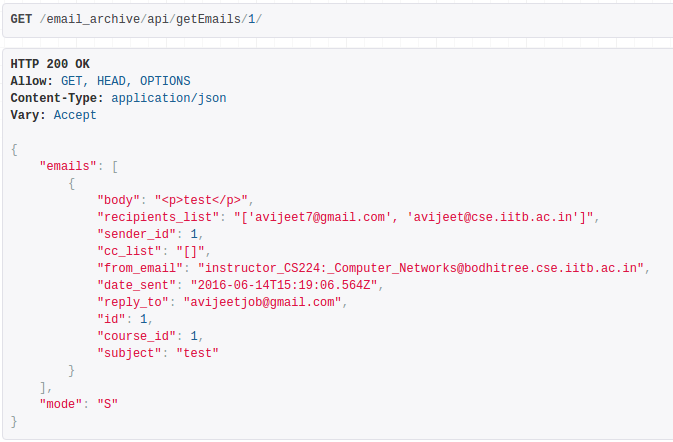
\includegraphics[width=0.95\linewidth]{./media/get_emails}
\caption{JSON returned by the \textit{getEmails} API}
\label{fig:get_emails}
\end{figure}

\subsubsection{UI for viewing the emails}

\begin{enumerate}
	\item React.js was used to create a component based design for viewing the archived emails. The emails are sorted such that the most recent will appear first.
	\item Each email is loaded as a separate expandable component1\textit{(html div)} which is initially collapsed, listing the sender and the subject of the email.
	\item Clicking on the sender or the subject expands the component to show the body of the email. Html emails are also rendered correctly in the body.
	\item An expandable recipients list is present which contains the email addresses of all the recipients. It is initially collapsed because in some cases the list may have a lot of addresses which would hinder viewability of the email.
\end{enumerate}

\begin{figure}[h]
\centering
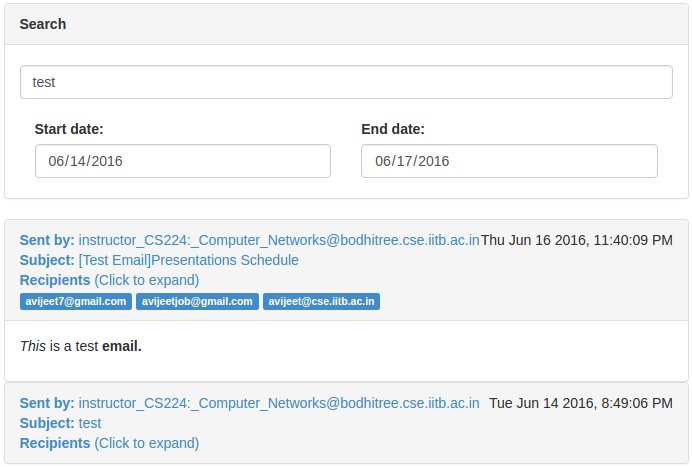
\includegraphics[width=0.95\linewidth]{./media/email_archive_ui}
\caption{UI for viewing the archived emails}
\label{fig:ea_ui}
\end{figure}

\subsubsection{Search and filter functions}

\begin{enumerate}
	\item An expandable container is present which contains the searchbox and date filter. 
	\item The searchbox provides \textit{``instant search''}, which means that the search will take place as the user is typing in the searchterm.
	\item The date filter is used to show only those emails that were sent between the start and the end dates specified in the filter.
\end{enumerate}

\subsection{Future Work}

\subsubsection{Pagination}

\hspace{0.35cm} Currently, all the emails are fetched using one database request and all of them are displayed on the email archive page. When the instructor sends a huge number of emails in a course, the list of emails will become undesirably long. In this case, there is need to paginate the results and display a certain amount of emails per page. The pages can also be fetched as and when requested.